\subsection{\texorpdfstring{Modeling of the QCD Background and $\Wen$ Signal Yield}{Modeling of the QCD Background and W-> e nu Signal Yield}}
\label{sec:WQCDbkg}

Three signal extraction methods are used, which give consistent
signal yields. The method described in Section~\ref{sec:AnalyticalFunction}
is used to extract the final result.

\subsubsection{Modeling the QCD Background Shape with an Analytical Function}
\label{sec:AnalyticalFunction}

The $\Wen$ signal is extracted using an unbinned maximum likelihood
(UML) fit to the $\MET$ distribution.
%Signal and EWK background
%distributions are derived from simulation and are validated using dedicated studies.

The shape of the $\MET$ distribution for the QCD background is modeled by a parametric function (modified Rayleigh
distribution) whose expression is
\begin{equation}
f_{\mathrm{QCD}}(\MET) = \MET\exp\left(-\frac{\MET{^2}}{2(\sigma_0+\sigma_1 \MET)^{2}}\right)\,.
\label{eq:rayleigh}
\end{equation}
The fit to a control sample, defined by inverting the track-cluster matching selection
variables $\Delta\eta$, $\Delta\phi$, shown in Fig.~\ref{fig:e-inverted}, illustrates
the quality of the description of the background shape by the parameterized function,
including the region of the signal, at high \MET.
\begin{figure}[htbp]
\begin{center}
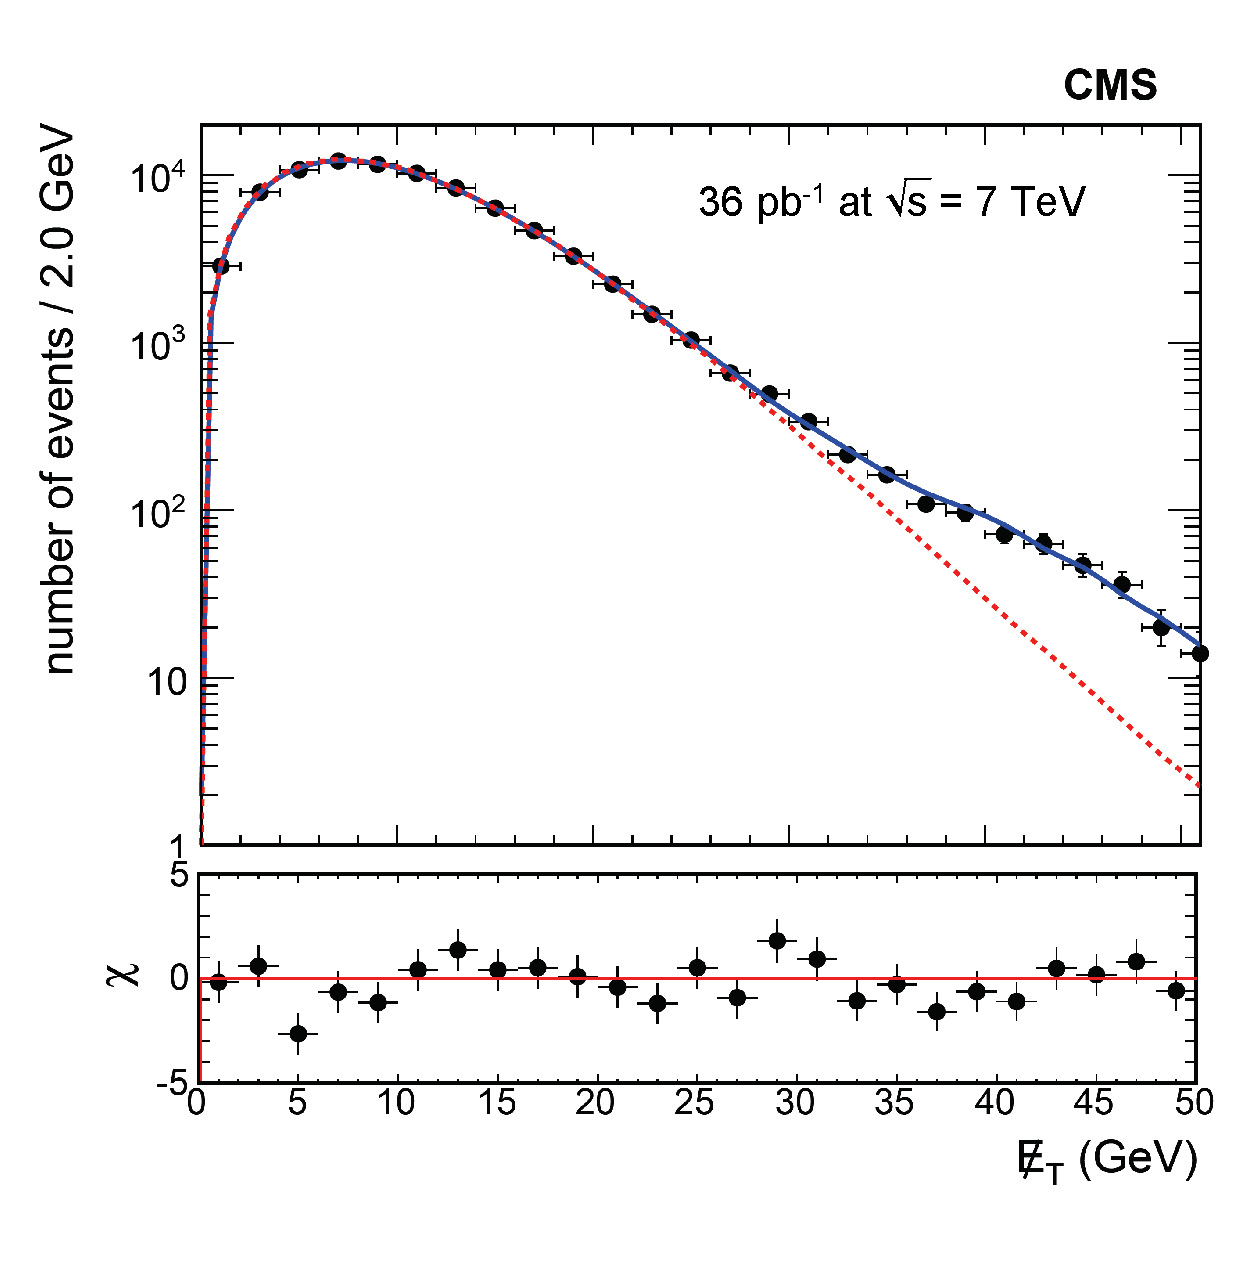
\includegraphics[width=0.50\textwidth]{figs/fixedMCyield_normal_model.pdf}
\caption{Fit to the background-dominated control sample defined by inverting
the selection on the track-match variables,
while maintaining the rest of the signal selection.
The blue solid line represents the model used to fit the control data sample. This is a Rayleigh
function plus a floating-yield signal shape that accounts for the signal contamination in the
control region. The magenta dashed line shows the Rayleigh function alone with its parameters estimated
from the combined fit.
}\label{fig:e-inverted}
\end{center}
\end{figure}
To study the systematic uncertainties associated with the background shape, the resolution term in
Eq.~(\ref{eq:rayleigh}) was changed by introducing an additional QCD shape parameter $\sigma_2$,
thus: $\sigma_0 + \sigma_1 \MET + \sigma_2 \MET^2$.

The free parameters of the UML fit are the QCD background yield,
the $\Wo$ signal yield, and the background shape
parameters $\sigma_0$ and $\sigma_1$.
The following signal yields are obtained:
$\WEIYIELD$ for the inclusive sample, $\WEPYIELD$ for the $\Wpen$ sample, and
$\WEMYIELD$ for the $\Wmen$ sample. 
The $\sigma_0$ and $\sigma_1$ values obtained from the fit are   
$\sigma_0$~=~8.56~$\pm$~0.15, $\sigma_1$~=~0.130~$\pm$~0.008 
for the $\Wpen$ sample, and $\sigma_0$~=~8.50~$\pm$~0.15, $\sigma_1$~=~0.139~$\pm$~0.008
for the $\Wmen$ sample. 
%with negligible correlation between the $\Wp$ and $\Wm$ yields.
The fit to the inclusive $\Wen$ sample is displayed
in Fig.~\ref{fig:Wen}, while the fits for the charge-specific
channels are displayed in Fig.~\ref{fig:WenPM}.

\begin{figure}[htbp]
\begin{center}
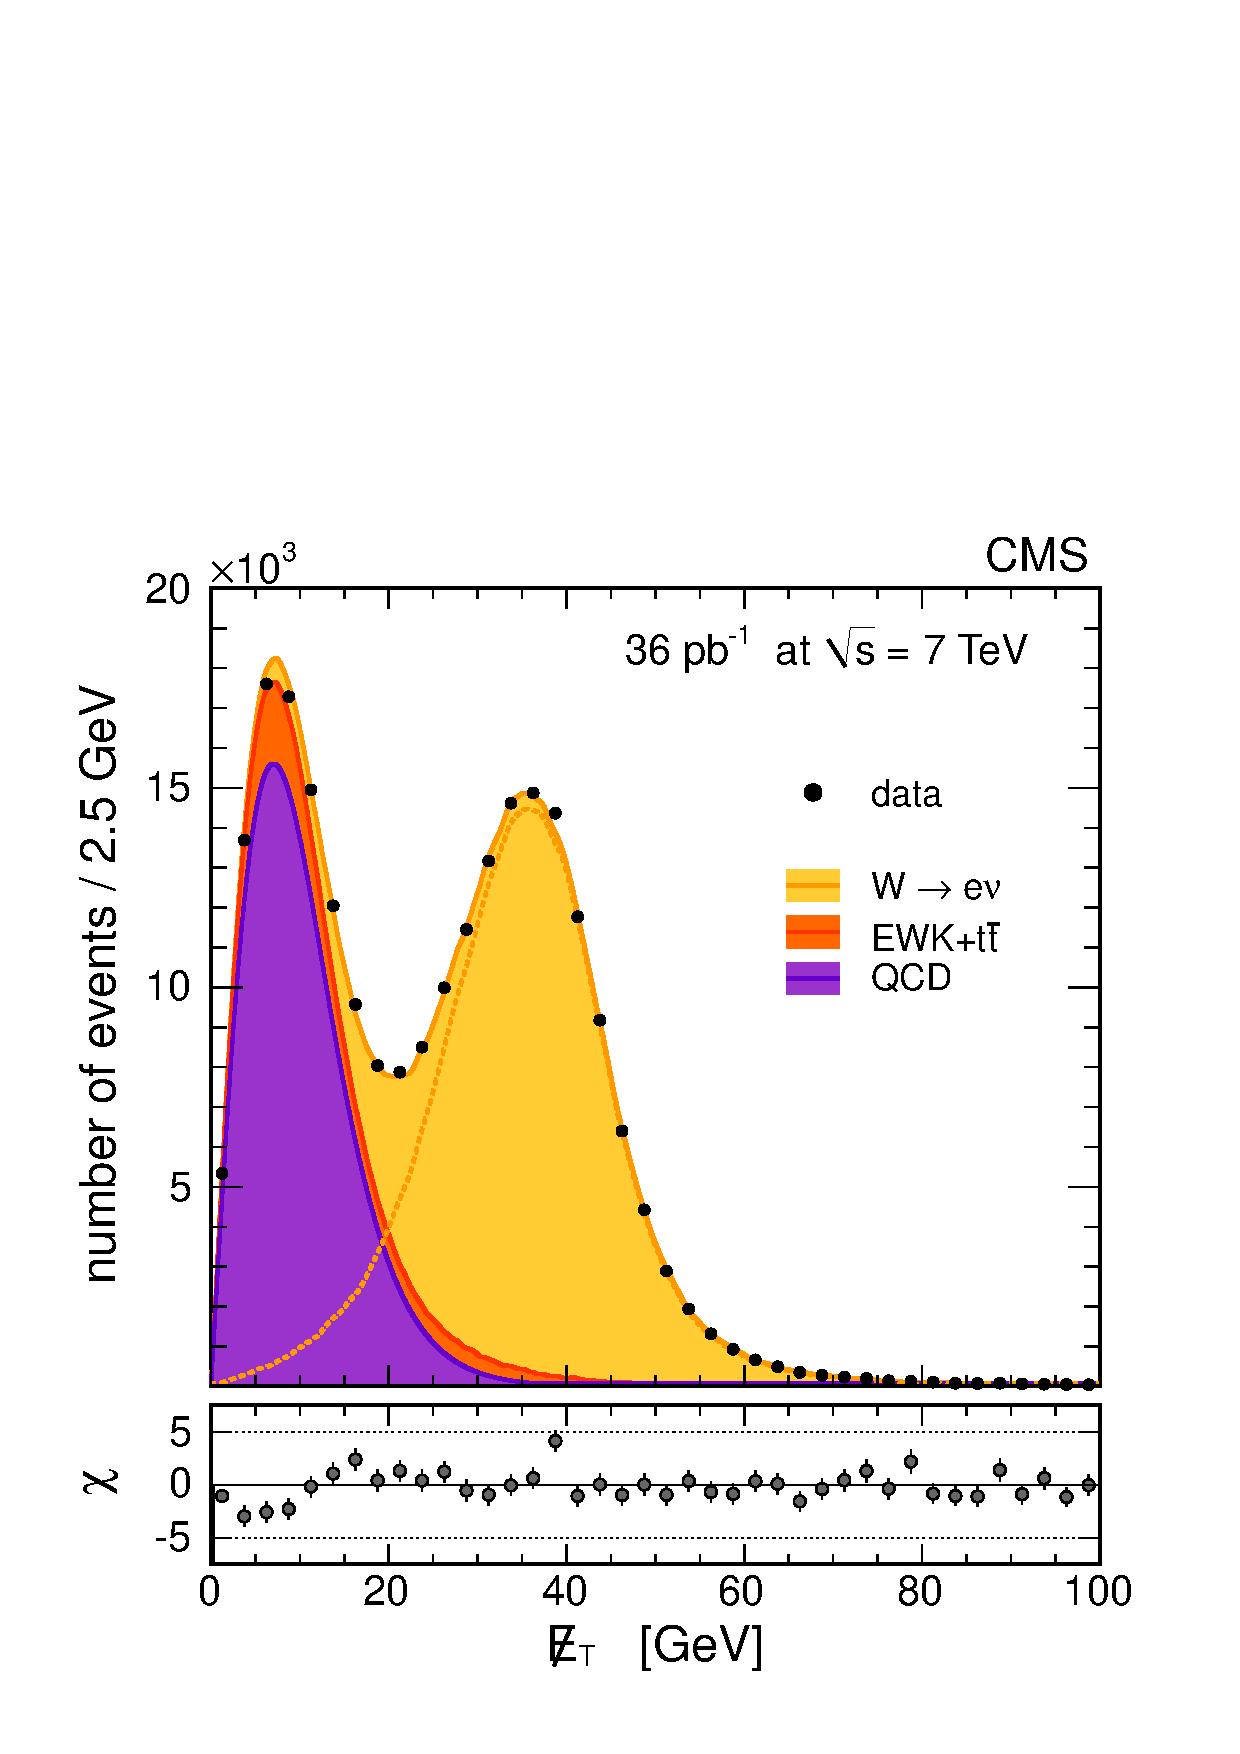
\includegraphics[width=0.48\textwidth]{figs/w_inc_36pb.pdf}
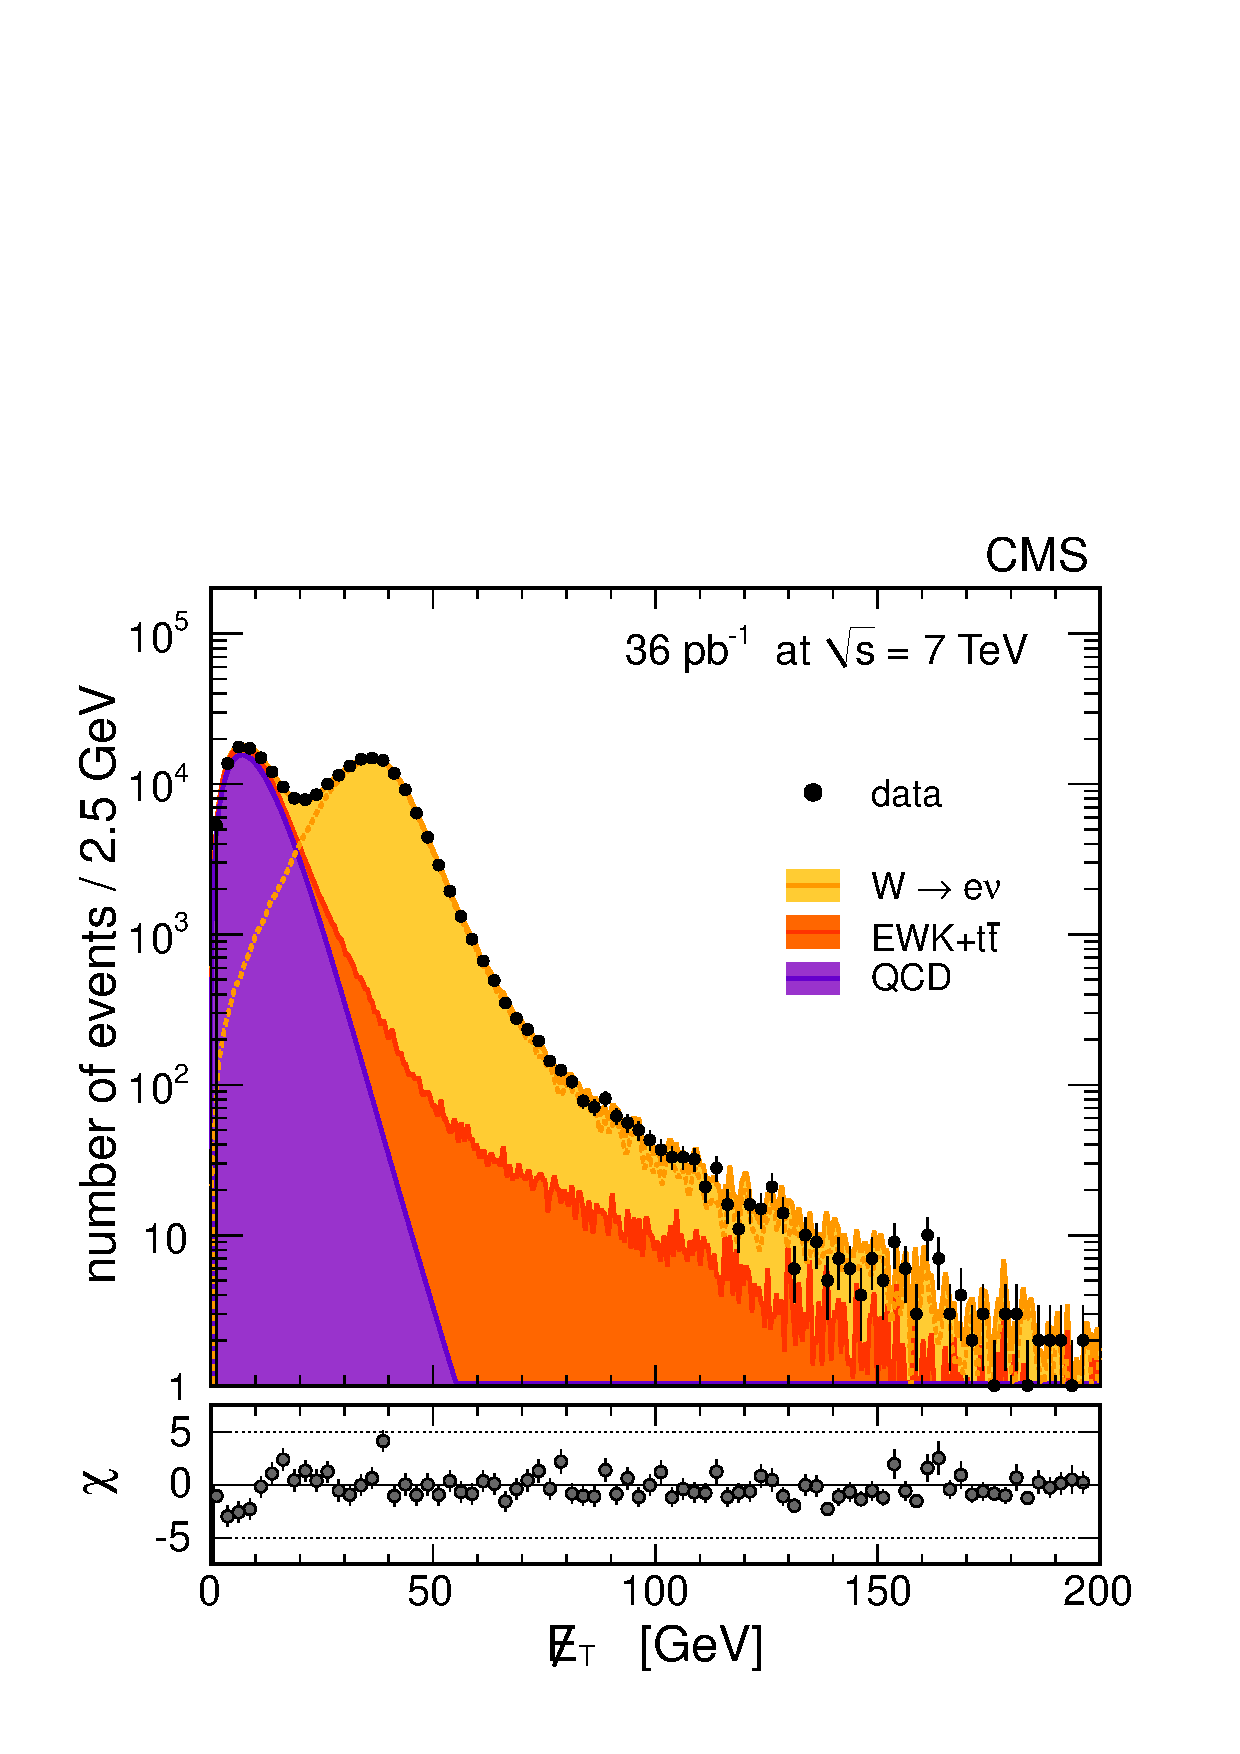
\includegraphics[width=0.48\textwidth]{figs/w_inc_36pb_log.pdf}
\caption{ \label{fig:Wen}
The $\MET$ distribution for the selected $\Wen$ candidates on
a linear scale (left) and on a logarithmic scale (right).
The points with the error bars represent the data. Superimposed are the
contributions obtained with the fit
for QCD background (violet, dark histogram), all other backgrounds
(orange, medium histogram), and signal plus  background (yellow, light histogram).
The orange dashed line is the fitted signal contribution.
}
\end{center}
\end{figure}

\begin{figure}[htbp]
\begin{center}
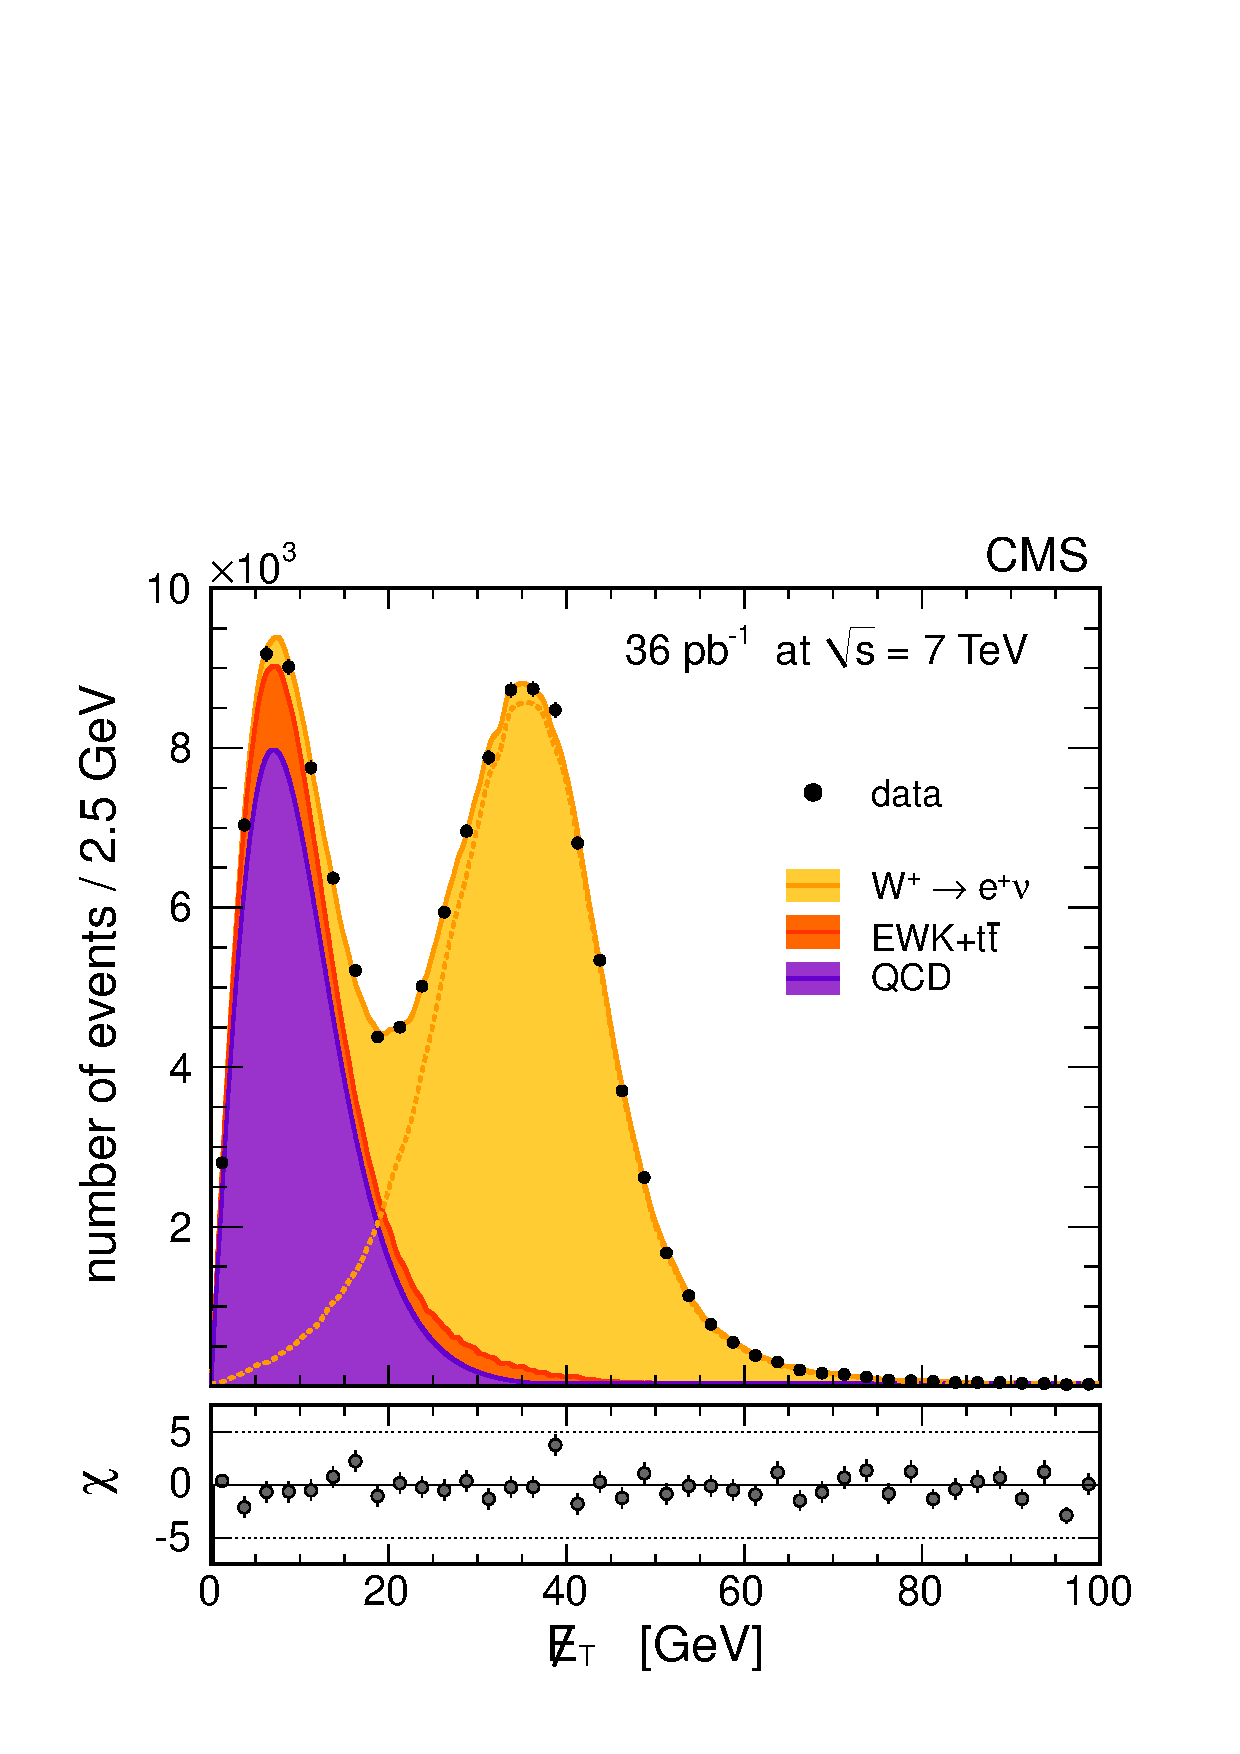
\includegraphics[width=0.48\textwidth]{figs/wp_36pb.pdf}
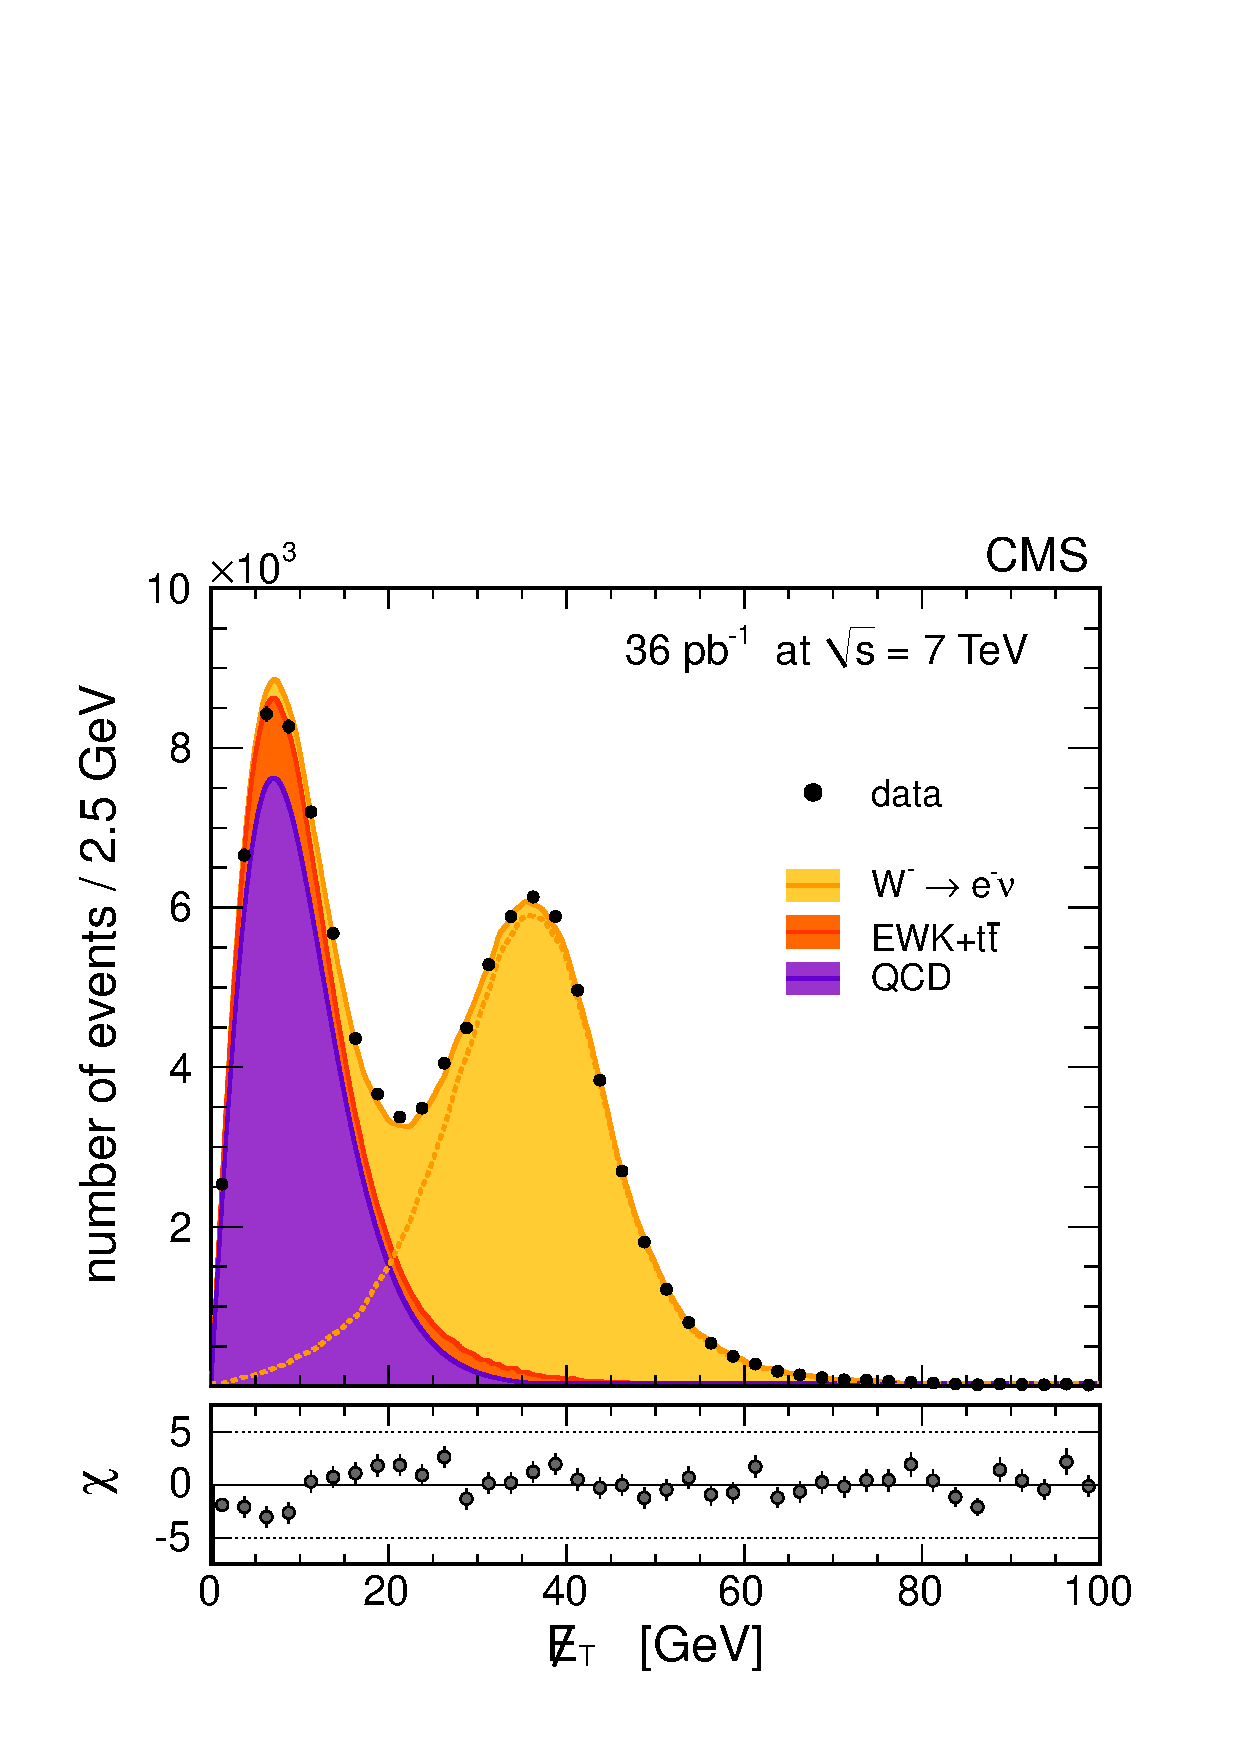
\includegraphics[width=0.48\textwidth]{figs/wm_36pb.pdf}
\caption{ \label{fig:WenPM}
The $\MET$ distributions for the selected W$^+$ (left) and W$^-$ (right) candidates.
The points with the error bars represent the data. Superimposed are the contributions
obtained with the fit for QCD background (violet, dark histogram), all other backgrounds
(orange, medium histogram), and signal plus background (yellow, light histogram).
The orange dashed line is the fitted signal contribution.
}
\end{center}
\end{figure}

The Kolmogorov--Smirnov probabilities for the fits to the charge-specific
channels are $\WEPKSPCOR$ for the $\Wp$ sample and
$\WEMKSPCOR$ for the $W^-$ sample.
\begin{figure}[t!]
\begin{center}
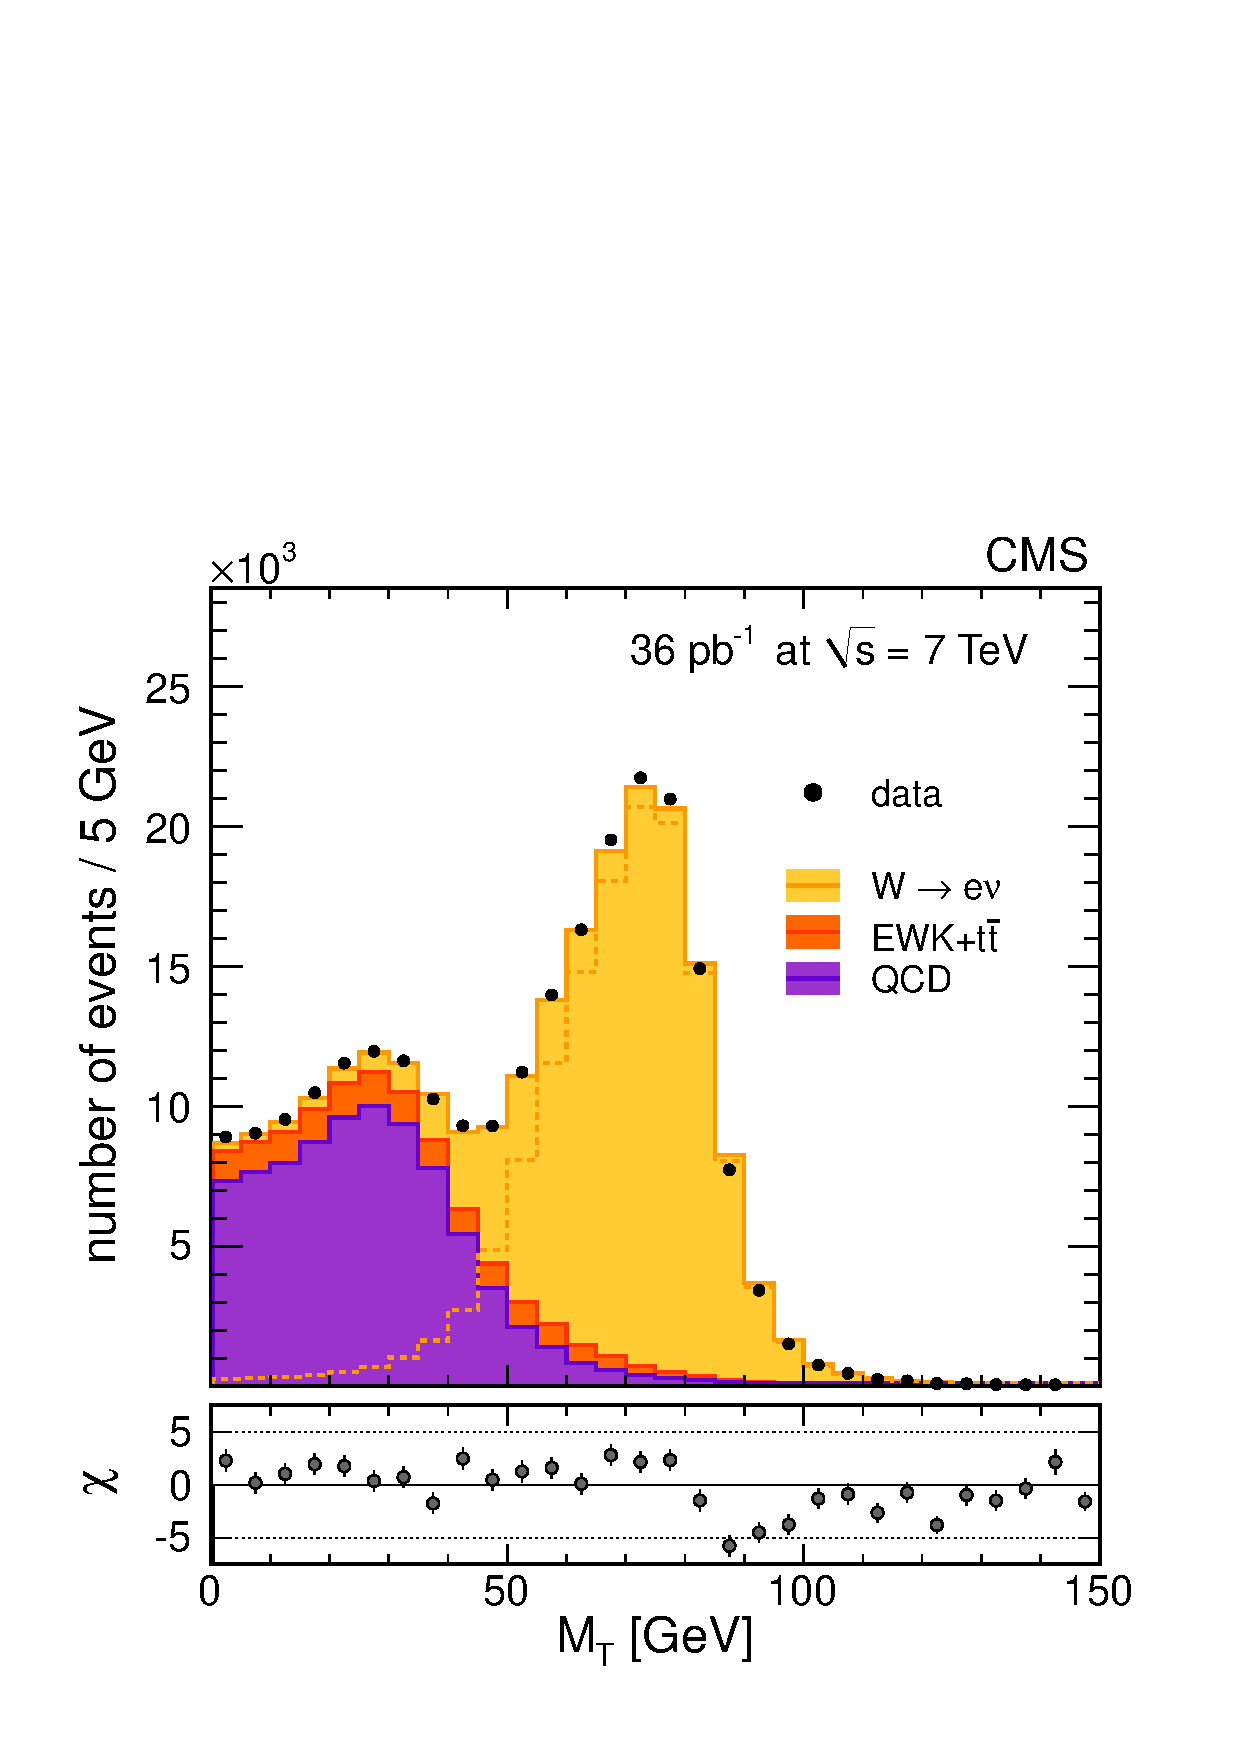
\includegraphics[width=0.48\textwidth]{figs/inc_pfmt_withMVA.pdf}
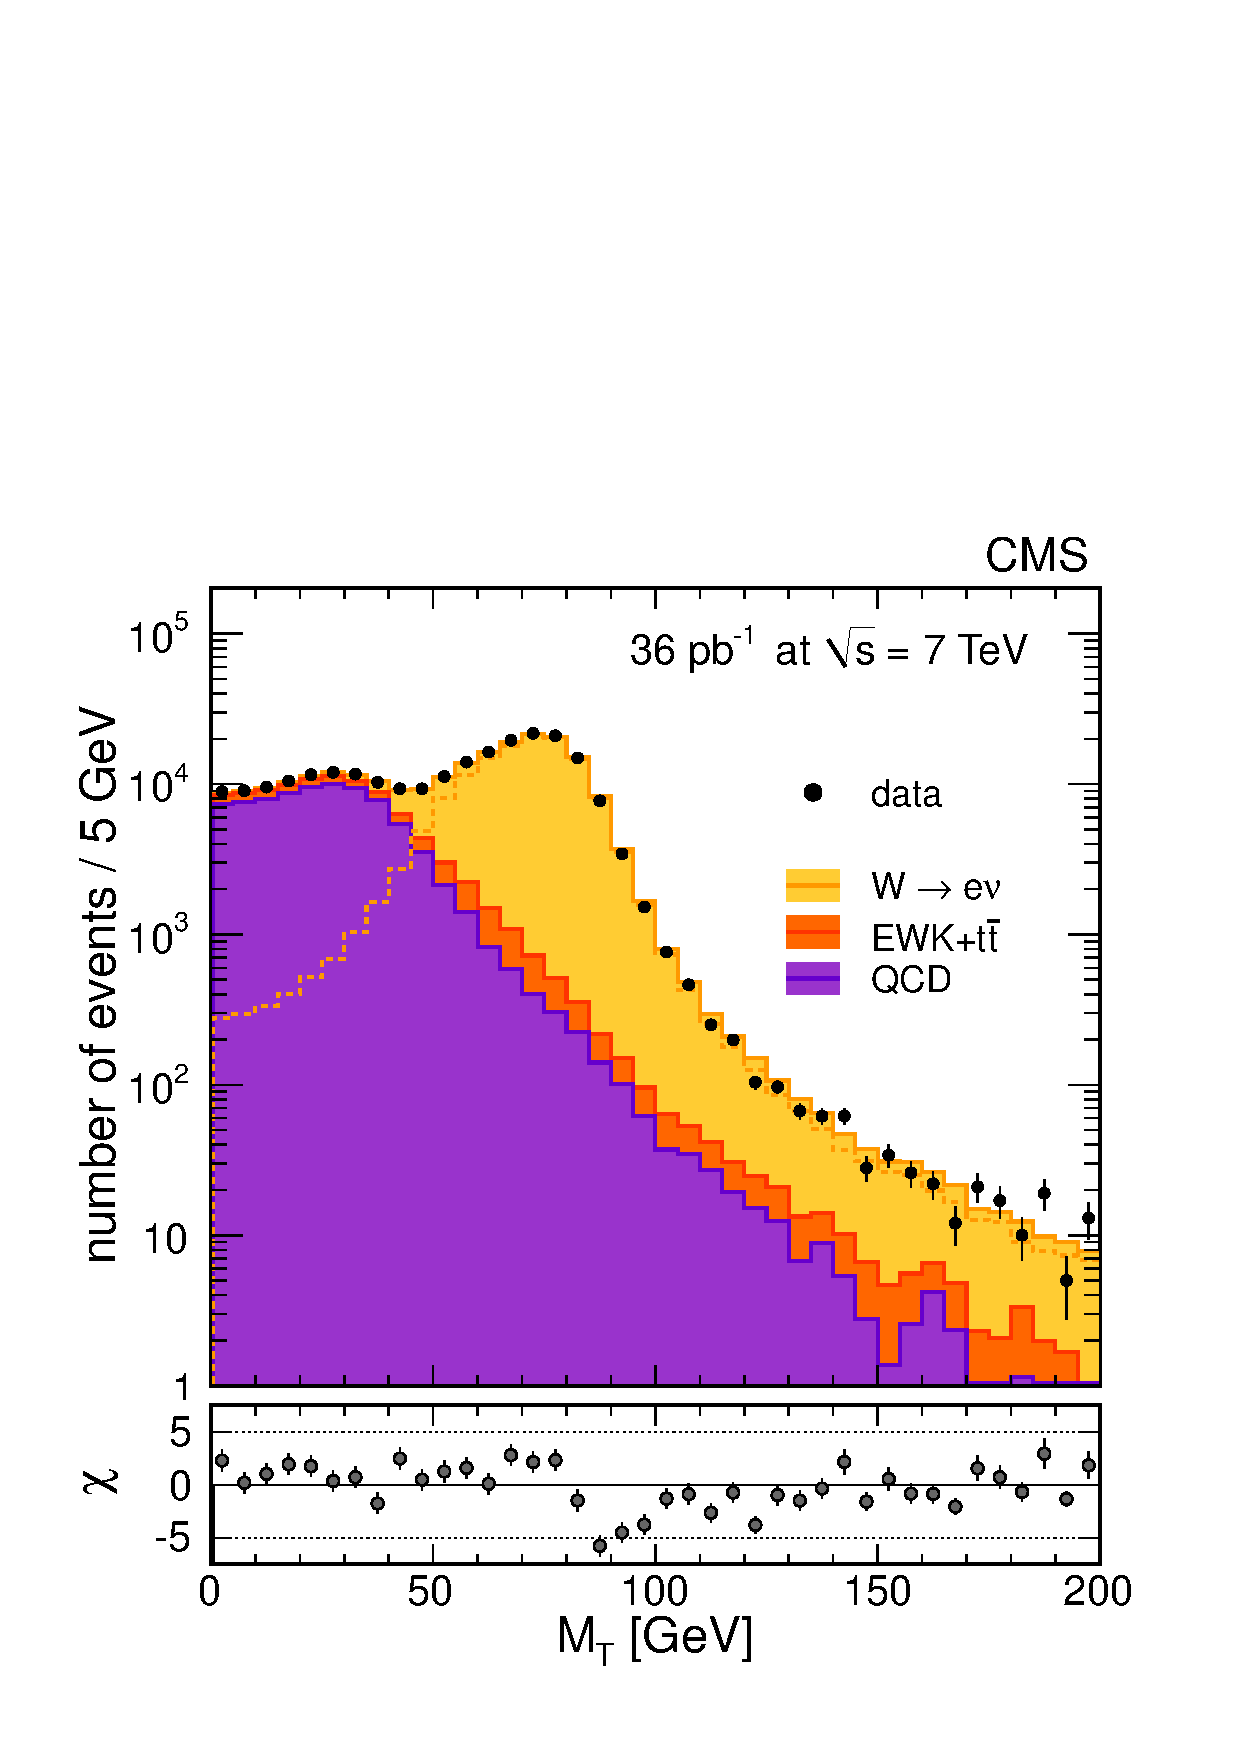
\includegraphics[width=0.48\textwidth]{figs/inc_pfmt_log_withMVA.pdf}
\caption{ \label{fig:WenMT}
The $\MT$ distribution for the selected $\Wen$ candidates on
a linear scale (left) and on a logarithmic scale (right).
The points with the error bars represent the data. Superimposed are the
contributions obtained with the fit
for QCD background (violet, dark histogram), all other backgrounds
(orange, medium histogram), and signal plus  background (yellow, light histogram).
The orange dashed line is the fitted signal contribution.
}
\end{center}
\end{figure}
Figure~\ref{fig:WenMT} shows the distribution for the inclusive $\Wo$ sample
of the transverse mass, defined as
$\MT=\sqrt{2\Pt\MET (1-\cos(\Delta\phi_{\mathrm{l},\MET}))}$,
where $\Delta\phi_{\mathrm{l},\MET}$ is the azimuthal angle between the
lepton and the $\MET$ directions.

\subsubsection{Modeling the QCD Background Shape with a Fixed Distribution}
\label{sec:e-Wsigextr-FixedTemplate}

In this approach the QCD shape is extracted directly from data using a 
control sample obtained by inverting a subset of the requirements used to select the 
signal. After fixing the shape from data,
only the normalization is allowed to float in the fit.  

The advantage of this approach 
is that detector effects, such as anomalous signals in the ca\-lo\-ri\-me\-ters or 
dead ECAL towers, are automatically reproduced in the QCD shape, since these 
effects are not affected by the selection inversion used to define the control sample.
The track-cluster matching variable $\Delta\eta$ is found
to have the smallest correlation with $\MET$ and is therefore chosen as the one 
to invert in order to suppress the signal and obtain the QCD control sample.  
Requirements on isolation and $H/E$ are the same as for the signal 
selection since these variables show significant correlation with \MET. 
\begin{figure}[h!]
  \begin{center}
    \includegraphics*[angle=-90,width=0.55\textwidth]{figs/antiselShape.pdf}
    \caption{Normalised \MET distribution for QCD and $\gamma$+jet simulated 
events passing the signal selection (solid histogram) compared 
to the normalised distribution for events from all simulated samples passing
the same inverted selection criteria used to obtain the control sample in data
(dashed histogram).}
    \label{fig:antiselShape}
  \end{center}
\end{figure}

The shape of the $\MET$ distribution for QCD and $\gamma$+jet simulated 
events passing the signal selection is compared 
to the \MET distribution for a simulated control sample composed of all simulated samples (signal and 
all backgrounds, weighted according to the 
theoretical production cross sections), after applying the same anti-selection 
as in data (Fig.~\ref{fig:antiselShape}).

\begin{figure}[htb]
  \begin{center}
    \includegraphics*[width=0.5\textwidth]{figs/Wenu_pfMET_lin.pdf}
%    \includegraphics*[width=0.48\textwidth]{figs/Wenu_pfMT_lin.pdf}
    \caption{Result of the fixed-shape fit to the $\MET$ distribution for all W candidates.
The points with the error bars represent the data.   Superimposed are the results
of the maximum likelihood fit for QCD background (violet, dark histogram), other backgrounds
(orange, medium histogram), and signal plus  background (yellow, light histogram).
The orange dashed line (left plot) is the fit contribution from signal.
}
    \label{fig:resultAll}
  \end{center}
\end{figure}

The difference in the $\MET$ distributions from the signal and inverted selections
is found to be predominantly due to two effects, which can be reduced by applying corrections.
The first effect is due to a large difference in the distribution of the output of a multivariate 
analysis (MVA) used for electron identification in the PF algorithm, between the selected events 
and the control sample. The value of the MVA output determines whether an electron candidate 
is treated by the PF algorithm as a genuine electron, or as a superposition of a charged pion and 
a photon, with track momentum and cluster energy each contributing separately to $\MET$. The control 
sample contains a higher fraction of electron candidates in the latter category, resulting in a bias on 
the $\MET$ shape. A correction is derived to account for this.
The second effect comes from the signal 
contamination in the control sample. The size of the contamination (1.17$\%$) is 
measured from data, using the \TNP technique with $\Zee$  
events, by measuring the efficiency for a signal electron to pass the 
control sample selection.


The results of the inclusive fit to the $\MET$ distribution with the fixed QCD background shape
are shown in Fig.~\ref{fig:resultAll}; the only free parameters in the extended 
maximum likelihood fit are the QCD and signal yields.
By applying this second method the following yields are obtained:
$135\,982 \pm 388$ (stat.) for the inclusive sample, $81\,286 \pm 302$ (stat.) for the $\Wpen$ sample, and
$54\,703 \pm 249$ (stat.) for the $\Wmen$ sample.
%with negligible correlation between the $\Wp$ and $\Wm$ yields.
%The quoted yields are from the $\MET$ fits. 
The ratios of the inclusive, $\Wpen$, and $\Wmen$ yields between this 
method and the parameterized
QCD shape method are $0.997 \pm 0.005$, $0.997 \pm 0.005$, and $0.999 \pm 0.005$, respectively, 
considering only the uncorrelated systematic uncertainties between the two methods.



\label{sec:e-Wsigextr-ABCDE}

\subsubsection{The ABCD Method}

%A brief summary of this method follows below. 
%A detailed description can be found 
%in the supporting document~\cite{CMS_AN_2011-009}.

In this method the data are divided into four categories defined by boundaries on $\MET$ and the relative tracker 
isolation, $\ITRK/\ET$, of the electron candidate. The boundaries of the regions are chosen to minimize the overall 
statistical and systematic uncertainties on the signal yield.
Values of $\MET$ above and below the boundary of 25 GeV, together with $\ITRK/\ET$ values below 
the boundary of 0.04, define the regions A and B, respectively.
\begin{figure}[htbp]
\begin{center}
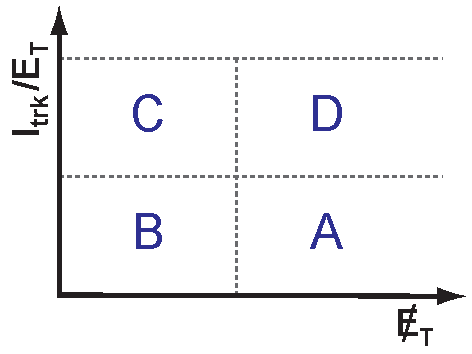
\includegraphics[width=0.35\textwidth]{figs/abcd.pdf}
\caption{The arrangement of the four categories of events used in the ABCD method. The vertical 
scale indicates increasing values of relative track isolation $\ITRK/\ET$
and the horizontal scale indicates increasing $\MET$.
%The dashed arrows show the directions of increasing signal purity.
}
\label{fig:abcde}
\end{center}
\end{figure}
Similarly, the regions above and below the $\MET$ boundary for $\ITRK/\ET$ values above 0.04, 
but below an upper $\ITRK/\ET$ bound of 0.2 (0.1) for electrons in the EB (EE), 
define the regions D and C, respectively. There is no upper bound for the $\MET$ values.
The different regions are shown graphically in Fig.~\ref{fig:abcde}, with region A 
having the greatest signal purity.
Combined regions are referred to as 'AB' (for A and B), for example.
The extracted signal corresponds to the entire ABCD region.

A system of equations is constructed relating the numbers of observed data events, $N_\mathrm{i}$, 
in each of the four regions ($\mathrm{i}$ = A, B, C and D) to the numbers 
of electroweak backgrounds, $E_\mathrm{i}$, QCD backgrounds, $Q_\mathrm{i}$, 
and signal events, $S_\mathrm{i}$. Several parameters should be determined from auxiliary 
measurements or simulations as shown in the following formulas: 

\begin{eqnarray}
 \label{eqABCD_Fa}
   f_\mathrm{A} & = & \frac{Q_\mathrm{A}}{Q_\mathrm{A} + Q_\mathrm{B}}  \\
  \label{eqABCD_Fb}
   f_\mathrm{D} & = & \frac{Q_\mathrm{D}}{Q_\mathrm{C} + Q_\mathrm{D}}  \\
  \label{eqABCD_EFFa}
   \epsilon_\mathrm{A} & = & \frac{S_\mathrm{A}}{S_\mathrm{A} + S_\mathrm{B}}  \\
  \label{eqABCD_EFFd}
   \epsilon_\mathrm{D} & = & \frac{S_\mathrm{D}}{S_\mathrm{C} + S_\mathrm{D}}  \\
  \label{eqABCD_EFFp}
   \epsilon_\mathrm{P} & = & \frac{S_\mathrm{A} + S_\mathrm{B}}{S_\mathrm{A} + S_\mathrm{B} + S_\mathrm{C} + S_\mathrm{D}} 
\end{eqnarray}

In this formulation, two parameters, $f_\mathrm{A}$ and $f_\mathrm{D}$, relate to the QCD 
backgrounds and are defined as the ratios of events with a fake electron candidate in the A and D 
regions to the number in the AB and CD regions, respectively. The two parameters represent the 
efficiency with which misidentified electrons pass the boundary on $\MET$ dividing
AD from BC. If the efficiency for passing the $\MET$ boundary is largely independent of the choice of
the boundaries on $\ITRK/\ET$, then these two parameters will be approximately equal. 
Assuming $f_\mathrm{A}=f_\mathrm{D}$ holds exactly 
leads to a simplification of the system of equations such that all direct dependence of the signal
extraction on parameters related to the QCD backgrounds is eliminated. For this idealized case there would be
no uncertainty on the extracted signal yield arising from modeling of QCD backgrounds. Detailed studies of the
data suggest this assumption holds to a good degree. A residual bias in the extracted signal arising from this
assumption is estimated directly from the data by studying a control sample 
obtained with inverted quality requirements on the electron candidate, 
and an appropriate small correction to the yield is applied (${\approx}0.37\%$).
A systematic uncertainty on the signal yield is derived from the uncertainty on this bias correction.
This contribution is small and is dominated by the uncertainty on signal
contamination in the control sample.

Three other important parameters relate to signal efficiencies: $\epsilon_\mathrm{A}$ 
and $\epsilon_\mathrm{D}$, which
are the efficiencies for signal events in the AB and CD regions, respectively, to pass the 
$\MET$ boundary, and $\epsilon_\mathrm{P}$, which is the efficiency for the electron candidate of a signal event 
to pass the boundary on relative track isolation dividing the AB region from the CD region under the 
condition that this electron already lies in the ABCD region. 
The first two of these, $\epsilon_\mathrm{A}$ and $\epsilon_\mathrm{D}$, are
estimated from models of the $\MET$ in signal events using the 
methods described in Section~\ref{sec:WsignalMETtemplate}.
The third parameter, $\epsilon_\mathrm{P}$, is measured from data using the \TNP method, described in
Section~\ref{sec:ELEefficiencies}, and is one of the dominant sources of 
uncertainty on the $\Wo$ boson yield before
considering the final acceptance corrections.

Electroweak background contributions are estimated from MC samples
with an overall normalization scaled through an iterative method with the signal yield. 
The electroweak contribution is subtracted from the observed data events in each of the four 
regions, $N_\mathrm{i} \rightarrow N_\mathrm{i} - E_\mathrm{i}$ ($\mathrm{i}$ = A, B, C and D).

Assuming that $f_\mathrm{A}$ = $f_\mathrm{B}$, the signal contained in the ABCD region, S, can 
be obtained from the following formula:

\begin{eqnarray}
 \label{eqABCD_S}
   \alpha S^2 + b S + c & = & 0 
\end{eqnarray}

with coefficients, 

\begin{eqnarray}
 \label{eqABCD_Sa}
   \alpha & = & \epsilon_\mathrm{P}(\epsilon_\mathrm{P} - 1)(\epsilon_\mathrm{A} - \epsilon_\mathrm{D})   \\
  \label{eqABCD_Sb}
   b & = & N_\mathrm{A}(1 - \epsilon_\mathrm{D})(1 - \epsilon_\mathrm{P}) - N_\mathrm{B}\epsilon_\mathrm{D}(1 - \epsilon_\mathrm{P}) + N_\mathrm{C}\epsilon_\mathrm{A}\epsilon_\mathrm{P} - N_\mathrm{D}\epsilon_\mathrm{P}(1 - \epsilon_\mathrm{A})  \\
  \label{eqABCD_Sc}
   c & = & N_\mathrm{B}N_\mathrm{D} - N_\mathrm{A}N_\mathrm{C}
\end{eqnarray}

The extracted yield with respect to the choice of boundaries in relative track isolation and $\MET$ is 
sensitive to biases in $\epsilon_\mathrm{P}$ and the QCD electron misidentification rate 
bias correction described above, respectively. 
The yield is very stable with respect to small changes in these selections, 
giving confidence that these 
important sources of systematic uncertainty are small.

The following signal yields are obtained:
$136\,003 \pm 498\,\mathrm{(stat.)}$ for the inclusive sample, $81\,525 \pm 385\,\mathrm{(stat.)}$ 
for the $\Wpen$ sample, and $54\,356 \pm 315\,\mathrm{(stat.)}$ for the $\Wmen$ sample.
%with negligible correlation between the $\Wp$ and $\Wm$ yields.
The ratios of the inclusive, $\Wpen$, and $\Wmen$ yields between this method and the parameterized
QCD shape are $0.998 \pm 0.007$, $0.999 \pm 0.007$, and $0.993 \pm 0.007$, respectively, considering
only the uncorrelated systematic uncertainties between the two methods.



The results of the three signal extraction methods are summarised in Table~\ref{tab:WsignalCollection}.

\begin{table}[htbp] %
\begin{center}
   \caption[.]{ \label{tab:WsignalCollection}
Comparison of $\Wen$ signal extraction methods. The signal yield of each method is presented together with
its statistical uncertainty.
For the fixed shape and the ABCD methods, the ratios of the signal yields with the analytical function method
are also shown taking into account only the uncorrelated systematics between the methods used in the ratios.}
\begin {tabular} {|l|l|c|c|c|}
\hline
\multicolumn{2}{|l|}{Source}        & $\Wen$           & $\Wpen$           & $\Wmen$            \\
\hline\hline
Analytical fun. &yield    & $\WEIYIELD$      &  $\WEPYIELD$      &  $\WEMYIELD$      \\
\hline
\multirow{2}{*}{Fixed shape} & yield                         & $\WEIftYIELD$    &  $\WEPftYIELD$    &  $\WEMftYIELD$      \\
 & ratio & $\rWEIftYIELD$   &  $\rWEPftYIELD$   &  $\rWEMftYIELD$      \\
\hline
\multirow{2}{*}{ABCD} & yield                                & $\WEIabYIELD$    & $\WEPabYIELD$     & $\WEMabYIELD$    \\
 & ratio       & $\rWEIabYIELD$   & $\rWEPabYIELD$    & $\rWEMabYIELD$    \\
\hline
\end {tabular}
\end{center}
\end{table}

